\documentclass{cubeamer}

\usepackage[french]{babel}
\usepackage[T1]{fontenc}
\usepackage{graphicx}

\title{Protection et gestion des licences}
\subtitle{Présentation - Gestion de projet}
\author{Sami Babigeon, Louka Boivin, Kaci Hammoudi, Alexis Osmont}
\date{\today}
\institute[Université de Rouen]{Master Informatique - 1ère année}

\begin{document}

\maketitle

\cutoc

%   Exemple de plan de présentation (mail de Karim)
%
%   Présentation du sujet et compréhension du besoin client
%   Périmètre fonctionnel à couvrir, appuyé par le diagramme global des cas d’utilisation
%   Solution technique argumentée avec diagramme d’architecture logicielle
%   Stratégie qualité pour la validation des livrables
%   Organisation du projet (i.e. affectation des rôles + découpage des tâches + stratégie de réalisation + organisation agile)
%   Planning du projet (i.e. focus sur les itérations > zoom sur le Gantt)
%   Principaux risques du projet et crédibilité de l'organisation mise en oeuvre
%
%   + POC si on a réussi

\section{Présentation du sujet}

\begin{frame}{Intitulé}
    \centerline{\textbf{Protection et gestion des licences}}
    \medskip
    \emph{Objectifs :}
    \begin{itemize}
        \item Génération et vérification des licences
        \item Plateforme de gestion pour le client, de demande pour les utilisateurs
        \item Protection des logiciels du client
    \end{itemize}
\end{frame}

\section{Analyse fonctionnel}

\begin{frame}{Besoin du client}
    Comment distribuer les logiciels que le client a développé ?
    \begin{itemize}
        \item Créer une licence unique pour une machine et un logiciel donné
        \item Une plateforme commune au client et aux utilisateurs
        \item Une libraire lui permettant d'intégrer la vérification à ses logiciels ou
            un outil permettant de greffer automatiquement
    \end{itemize}
\end{frame}

\begin{frame}{Cas d'utilisations}
    \begin{figure}
        \centering
        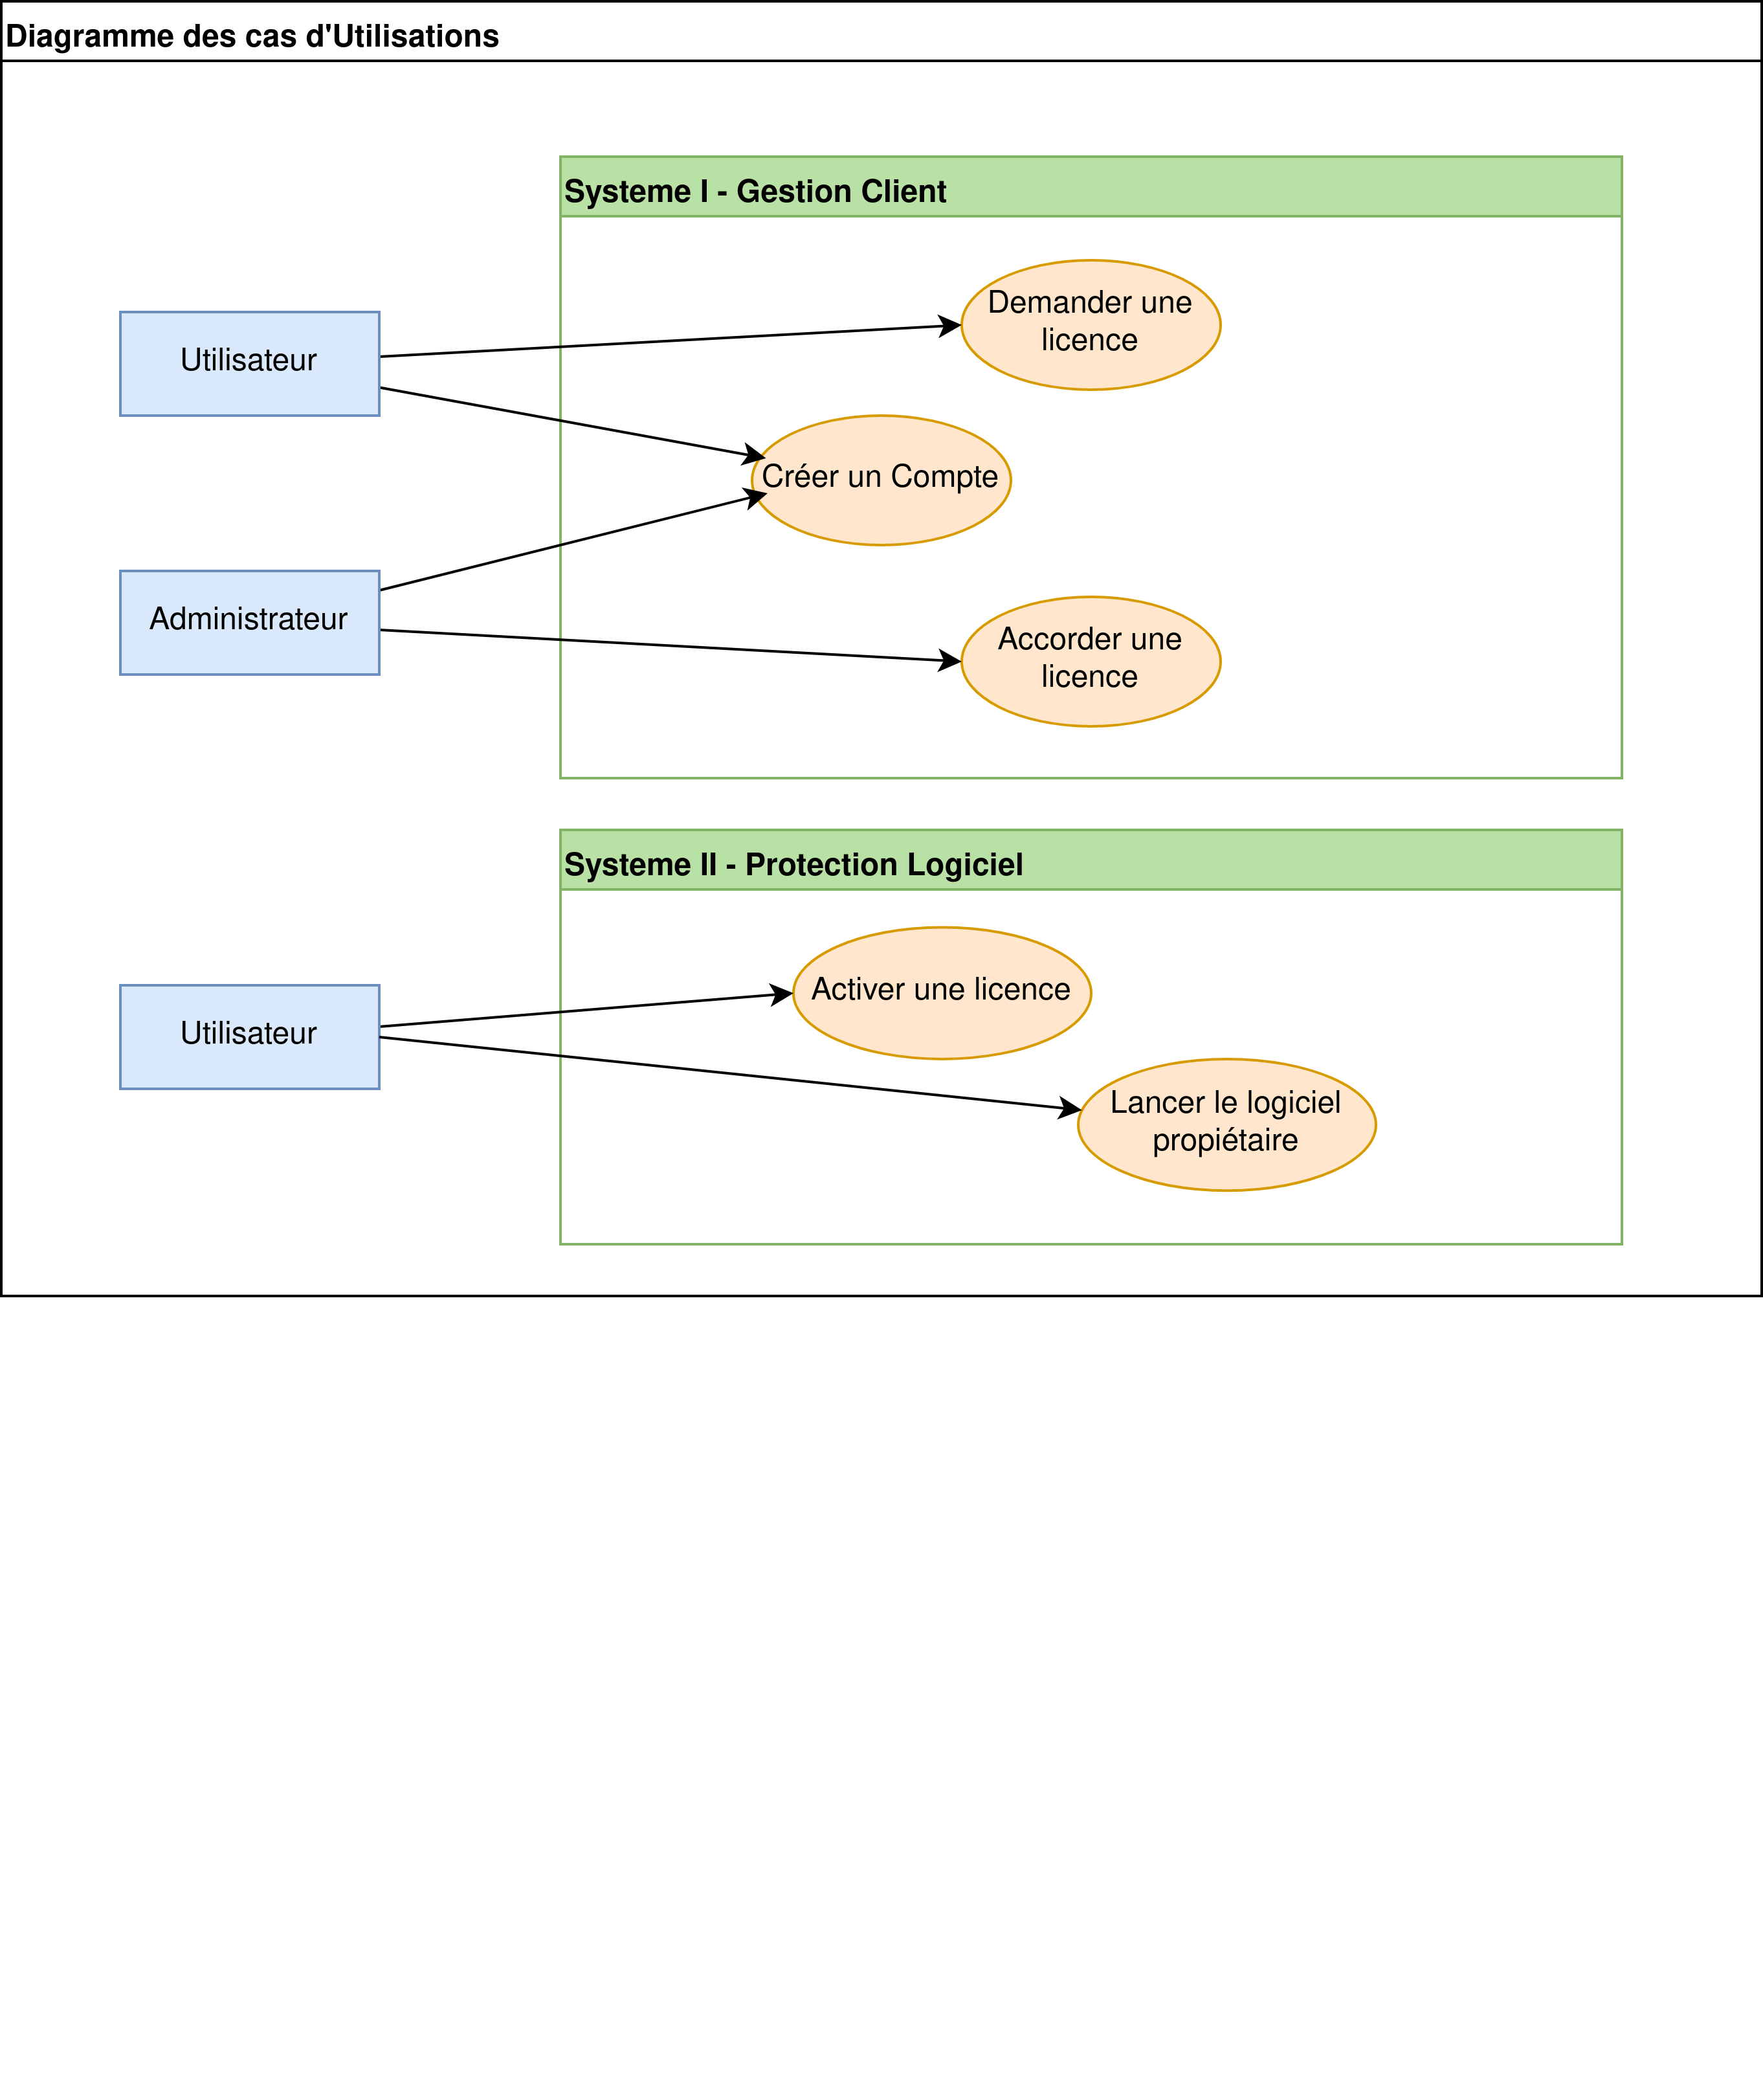
\includegraphics[scale=0.5]{img/Util.png}
    \end{figure}
\end{frame}

\begin{frame}{Exigences}
    \begin{itemize}
        \item Sécurité
        \medskip
        \item Compatibilité Windows
        \medskip
        \item Maintenabilité
    \end{itemize}
\end{frame}

%    \begin{tikzpicture}
%        \draw (0,0) ellipse (1.5cm and 0.5cm) node[black,fill=white]{Chiffrement};
%        \draw (3,0) ellipse (1.5cm and 0.5cm) node[black,fill=white]{PBKDF};
%        \draw (7,0) ellipse (1.8cm and 0.5cm) node[black,fill=white]{Base de données};
%        \draw (11,0) ellipse (1.5cm and 0.5cm) node[black,fill=white]{Obfuscation};
%    \end{tikzpicture}
%    \begin{tikzpicture}
%        \draw (5,0) ellipse (1.8cm and 0.5cm) node[black,fill=white]{Documentation};
%        \draw (10,0) ellipse (1.8cm and 0.5cm) node[black,fill=white]{Charte de code};
%    \end{tikzpicture}
%     \begin{tikzpicture}
%        \draw (3,0) ellipse (2cm and 0.5cm) node[black,fill=white]{Tests sur Windows};
%        \draw (7,0) ellipse (1.2cm and 0.5cm) node[black,fill=white]{DLL};
%        \draw (10,0) ellipse (1.5cm and 0.5cm) node[black,fill=white]{Injection PE};
%    \end{tikzpicture}

\begin{frame}{Fonctionnement globale}
    \begin{figure}
        \centering
        \vspace{-0.1cm}
        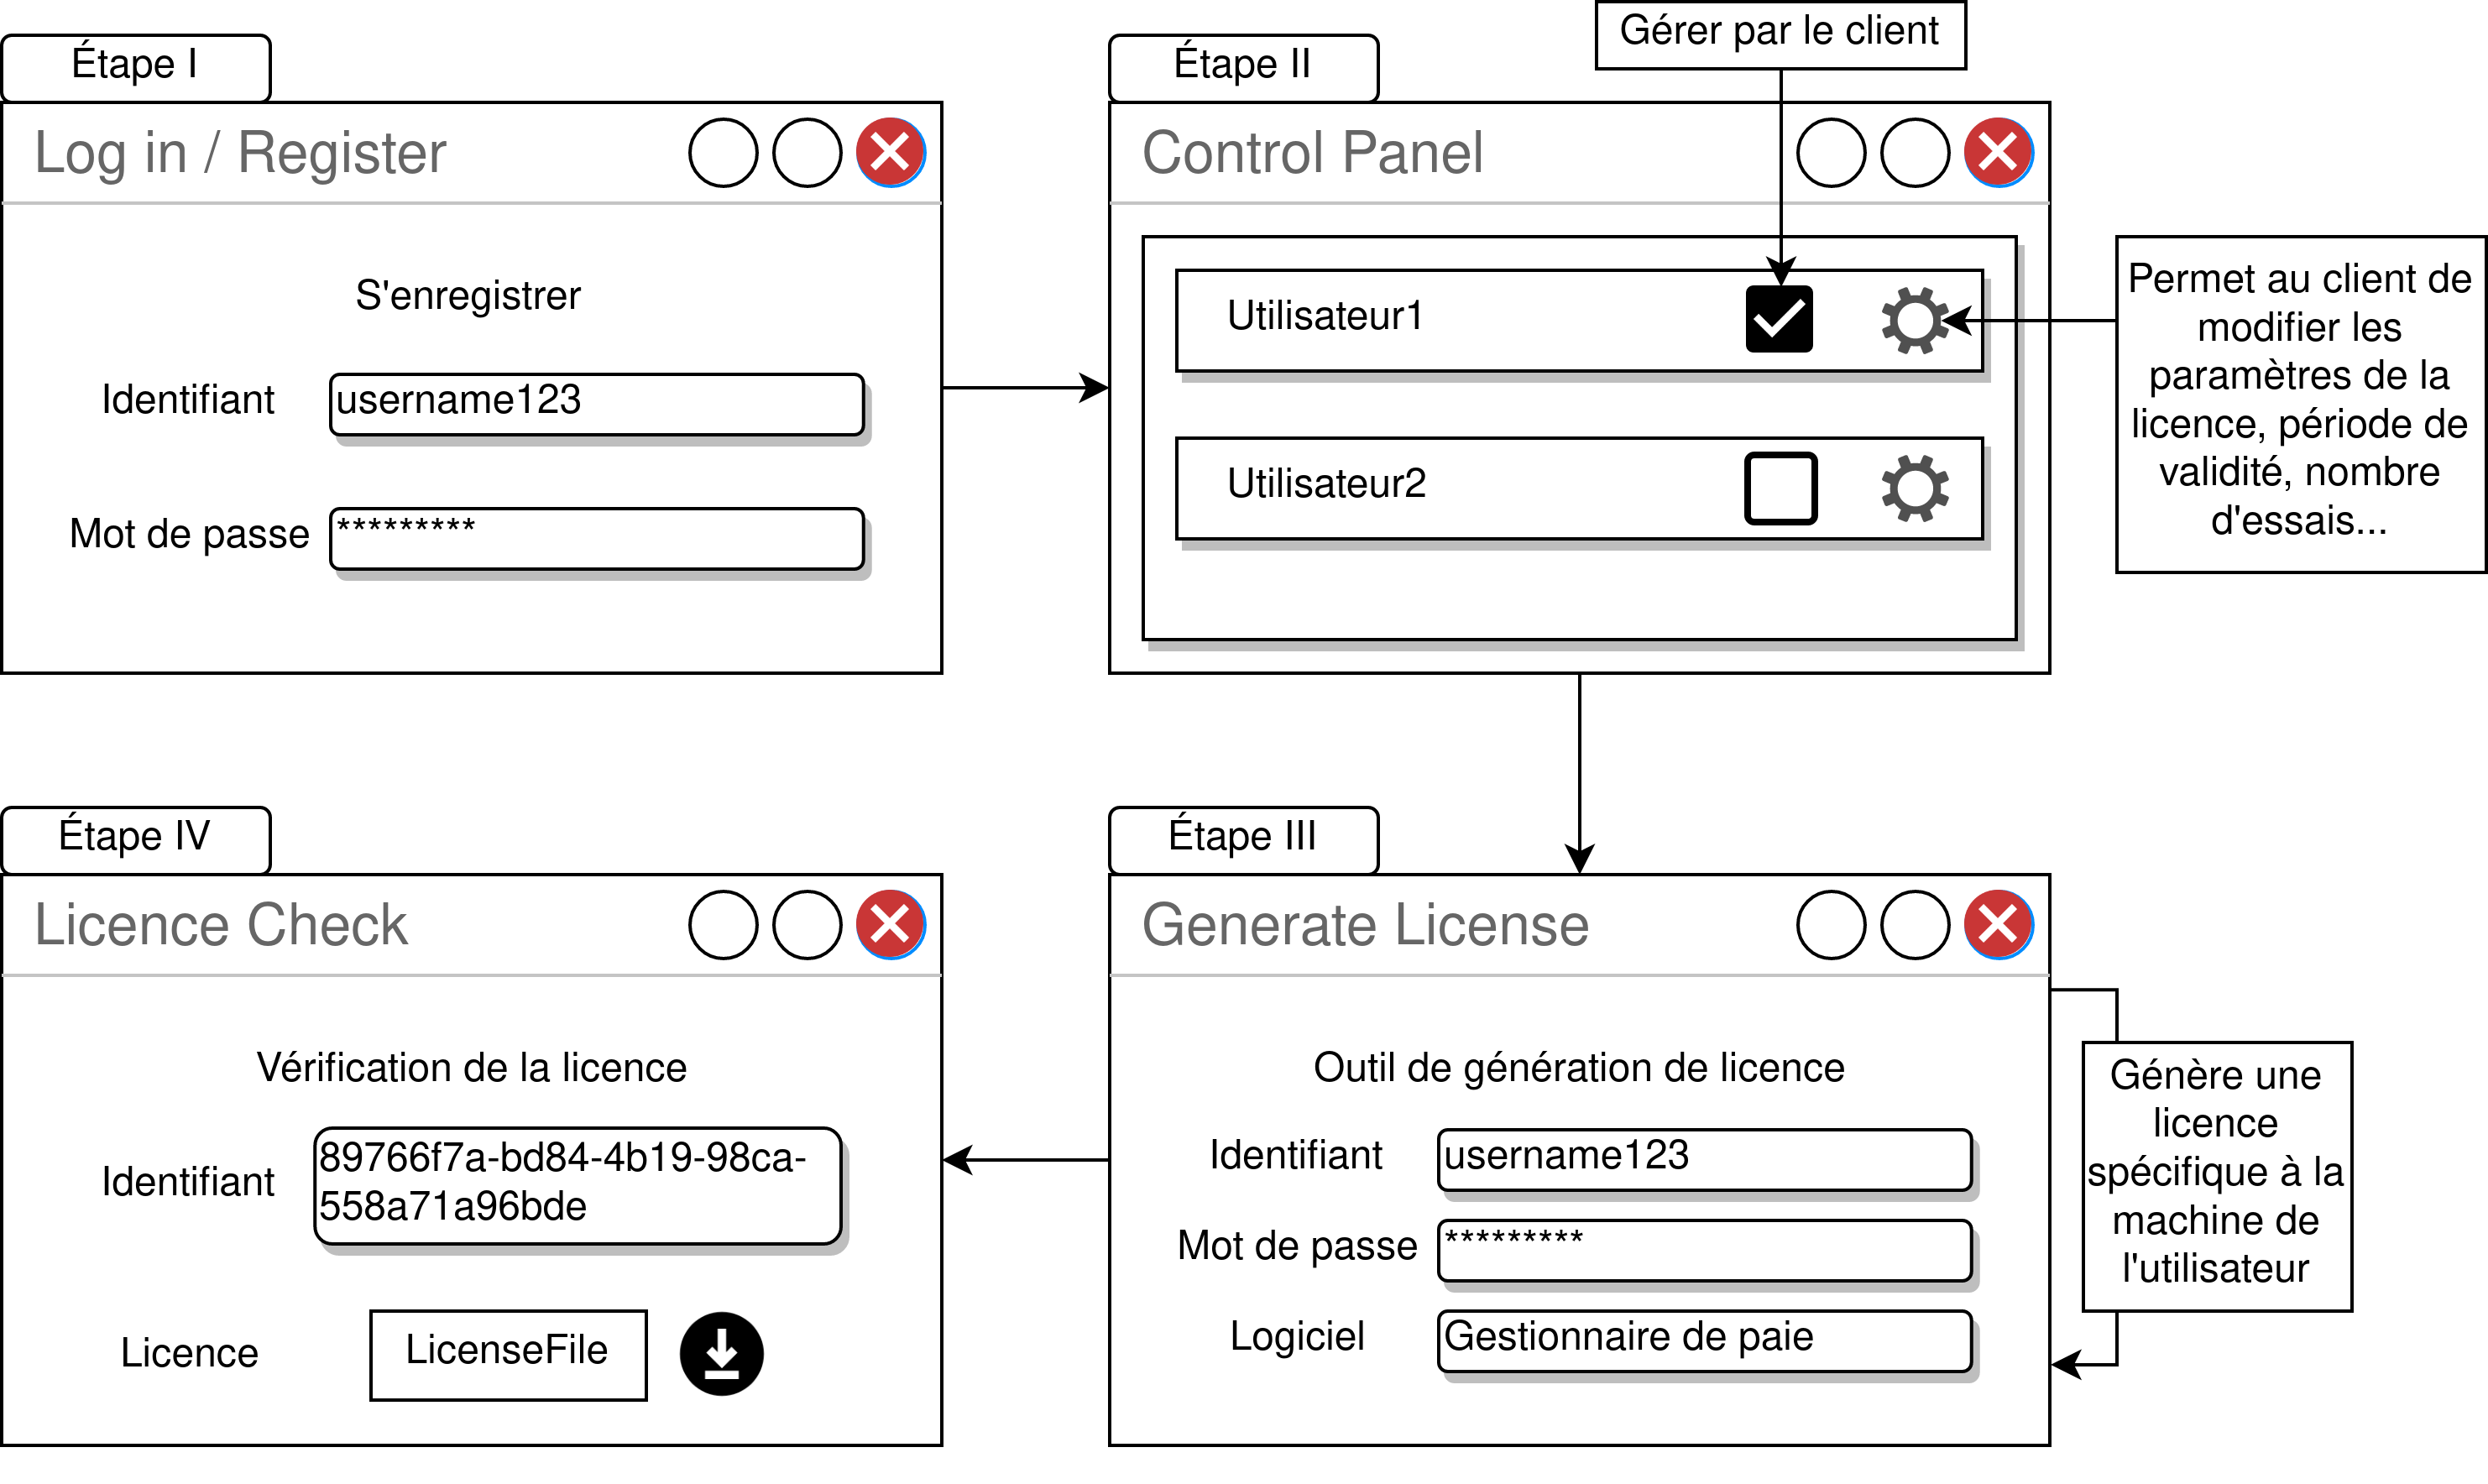
\includegraphics[scale=0.58]{img/STB.png}
    \end{figure}
\end{frame}

\section{Solution technique}

\begin{frame}{Architecture logicielle - Serveur}
    \begin{figure}
        \centering
        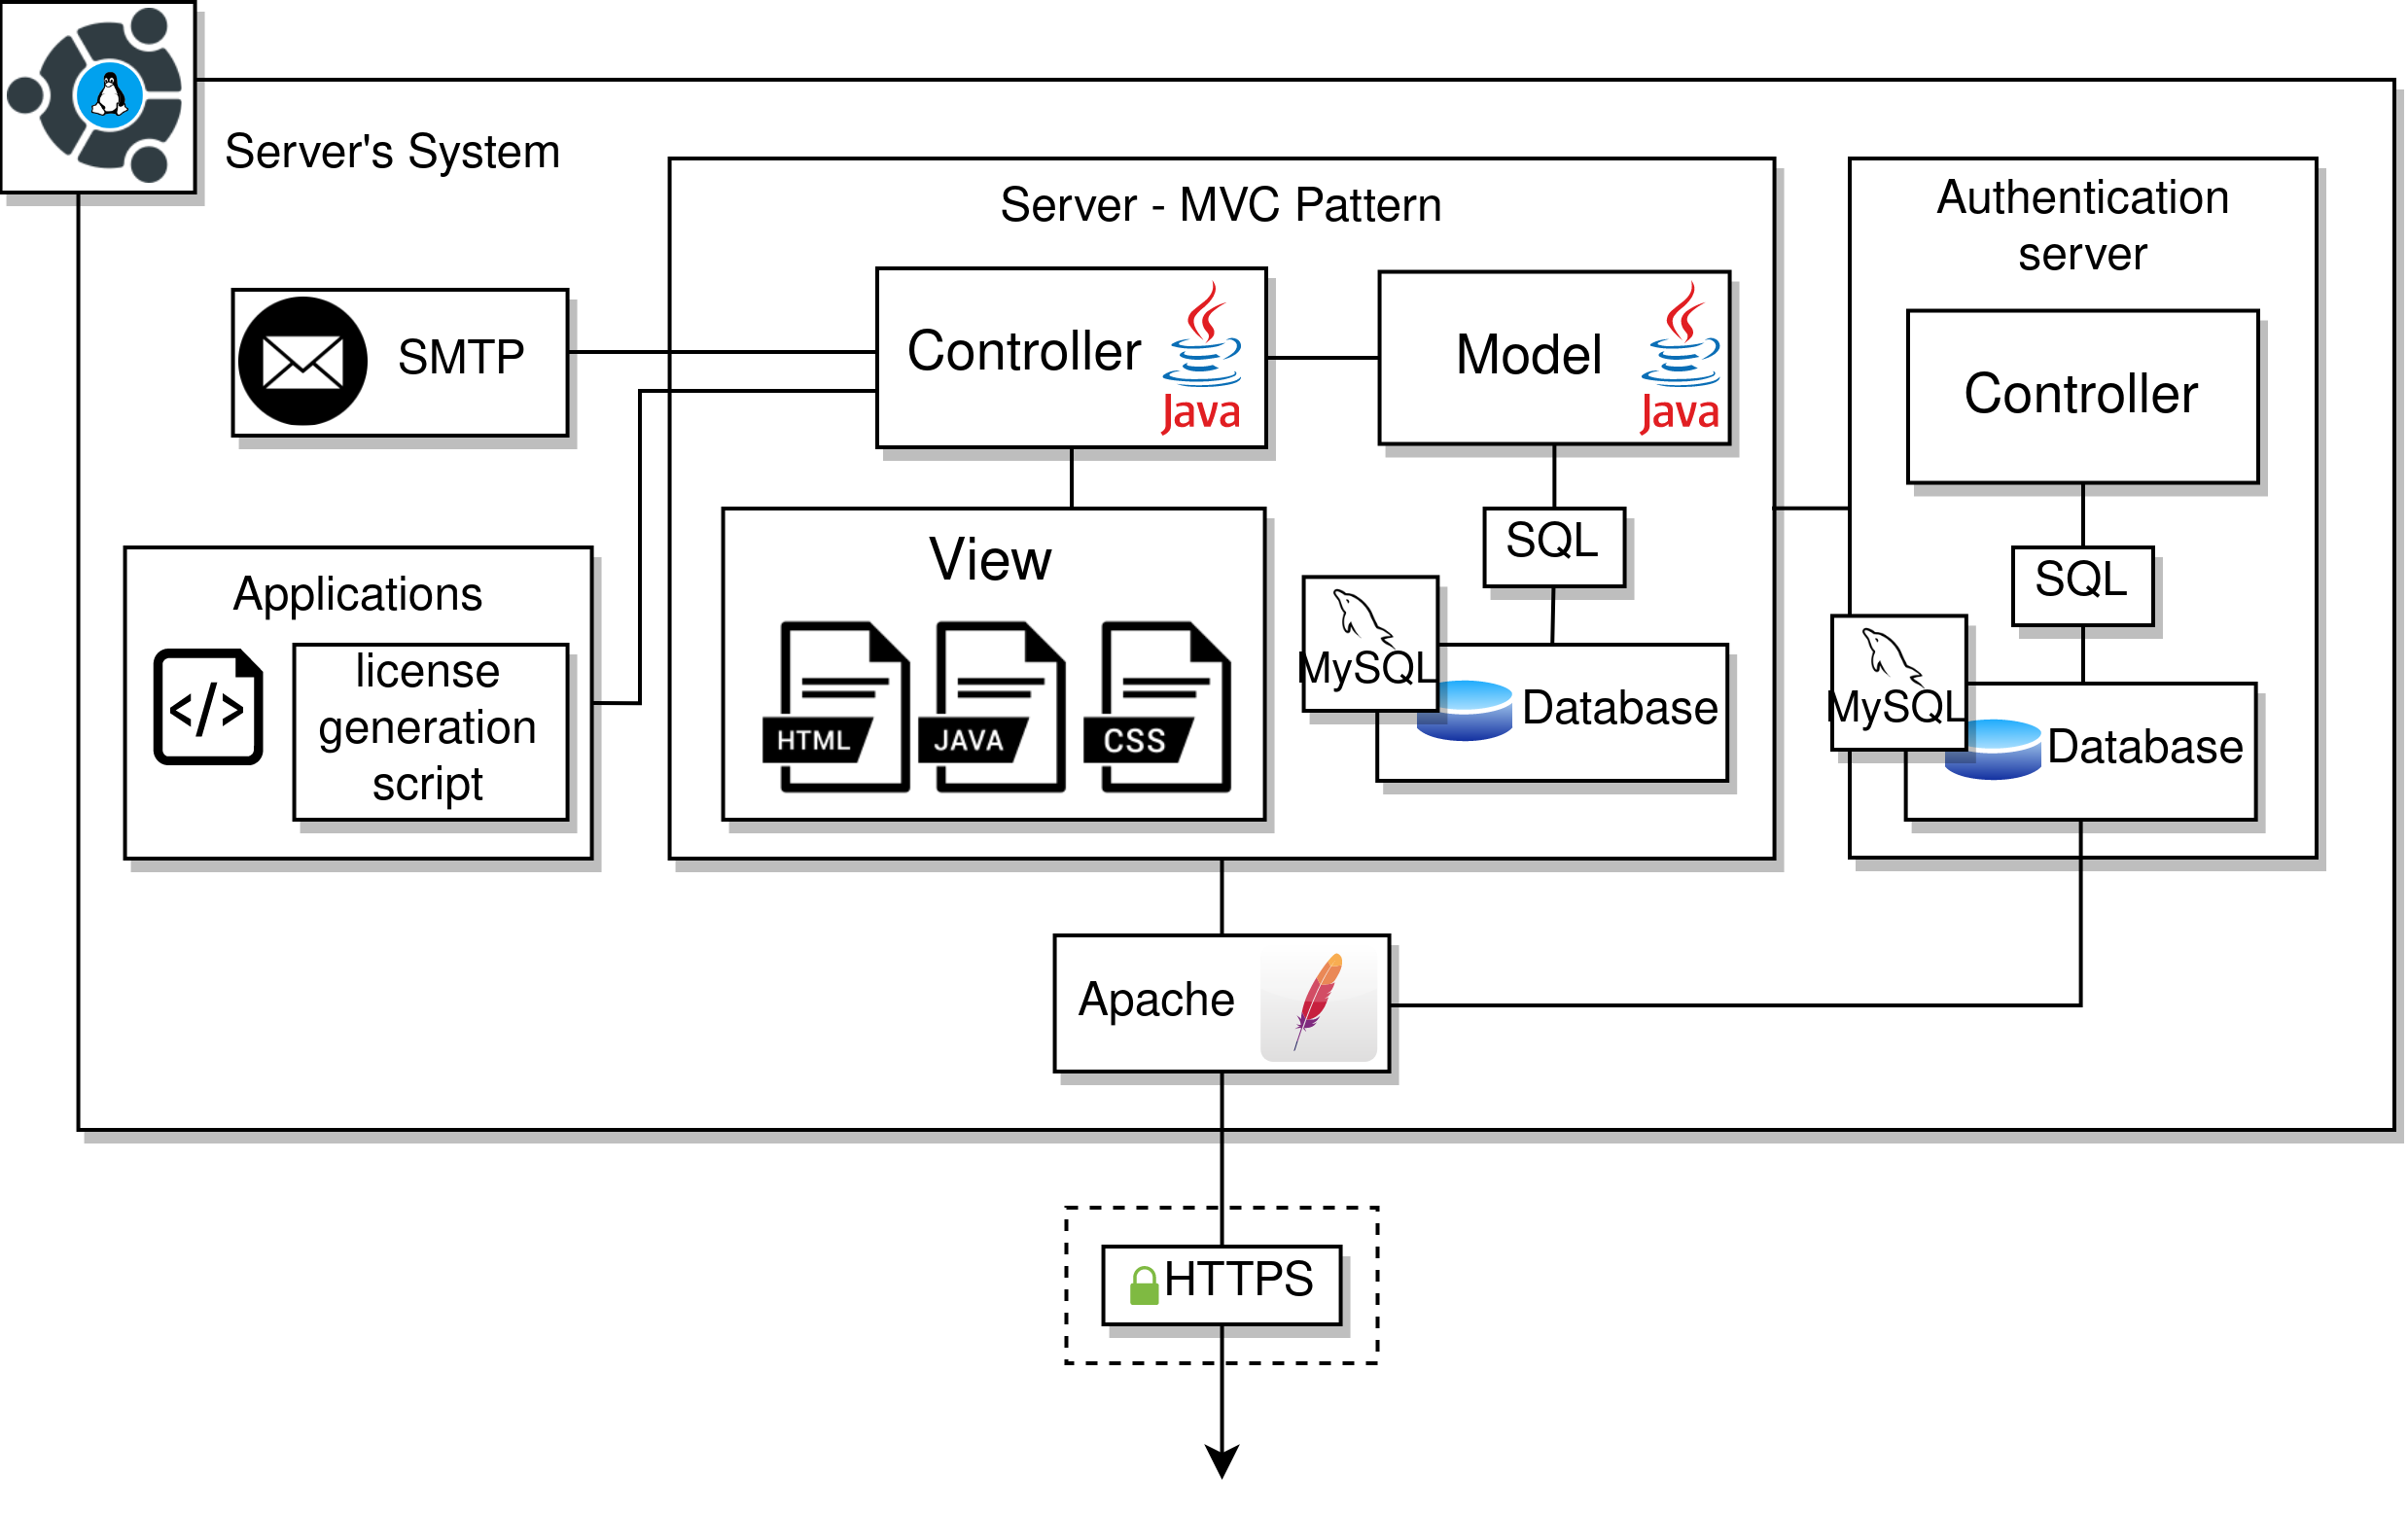
\includegraphics[scale=0.7]{img/DAT-server.png}
    \end{figure}
\end{frame}

\begin{frame}{Architecture logicielle - Client}
    \begin{figure}
        \centering
        \vspace{-0.8cm}
        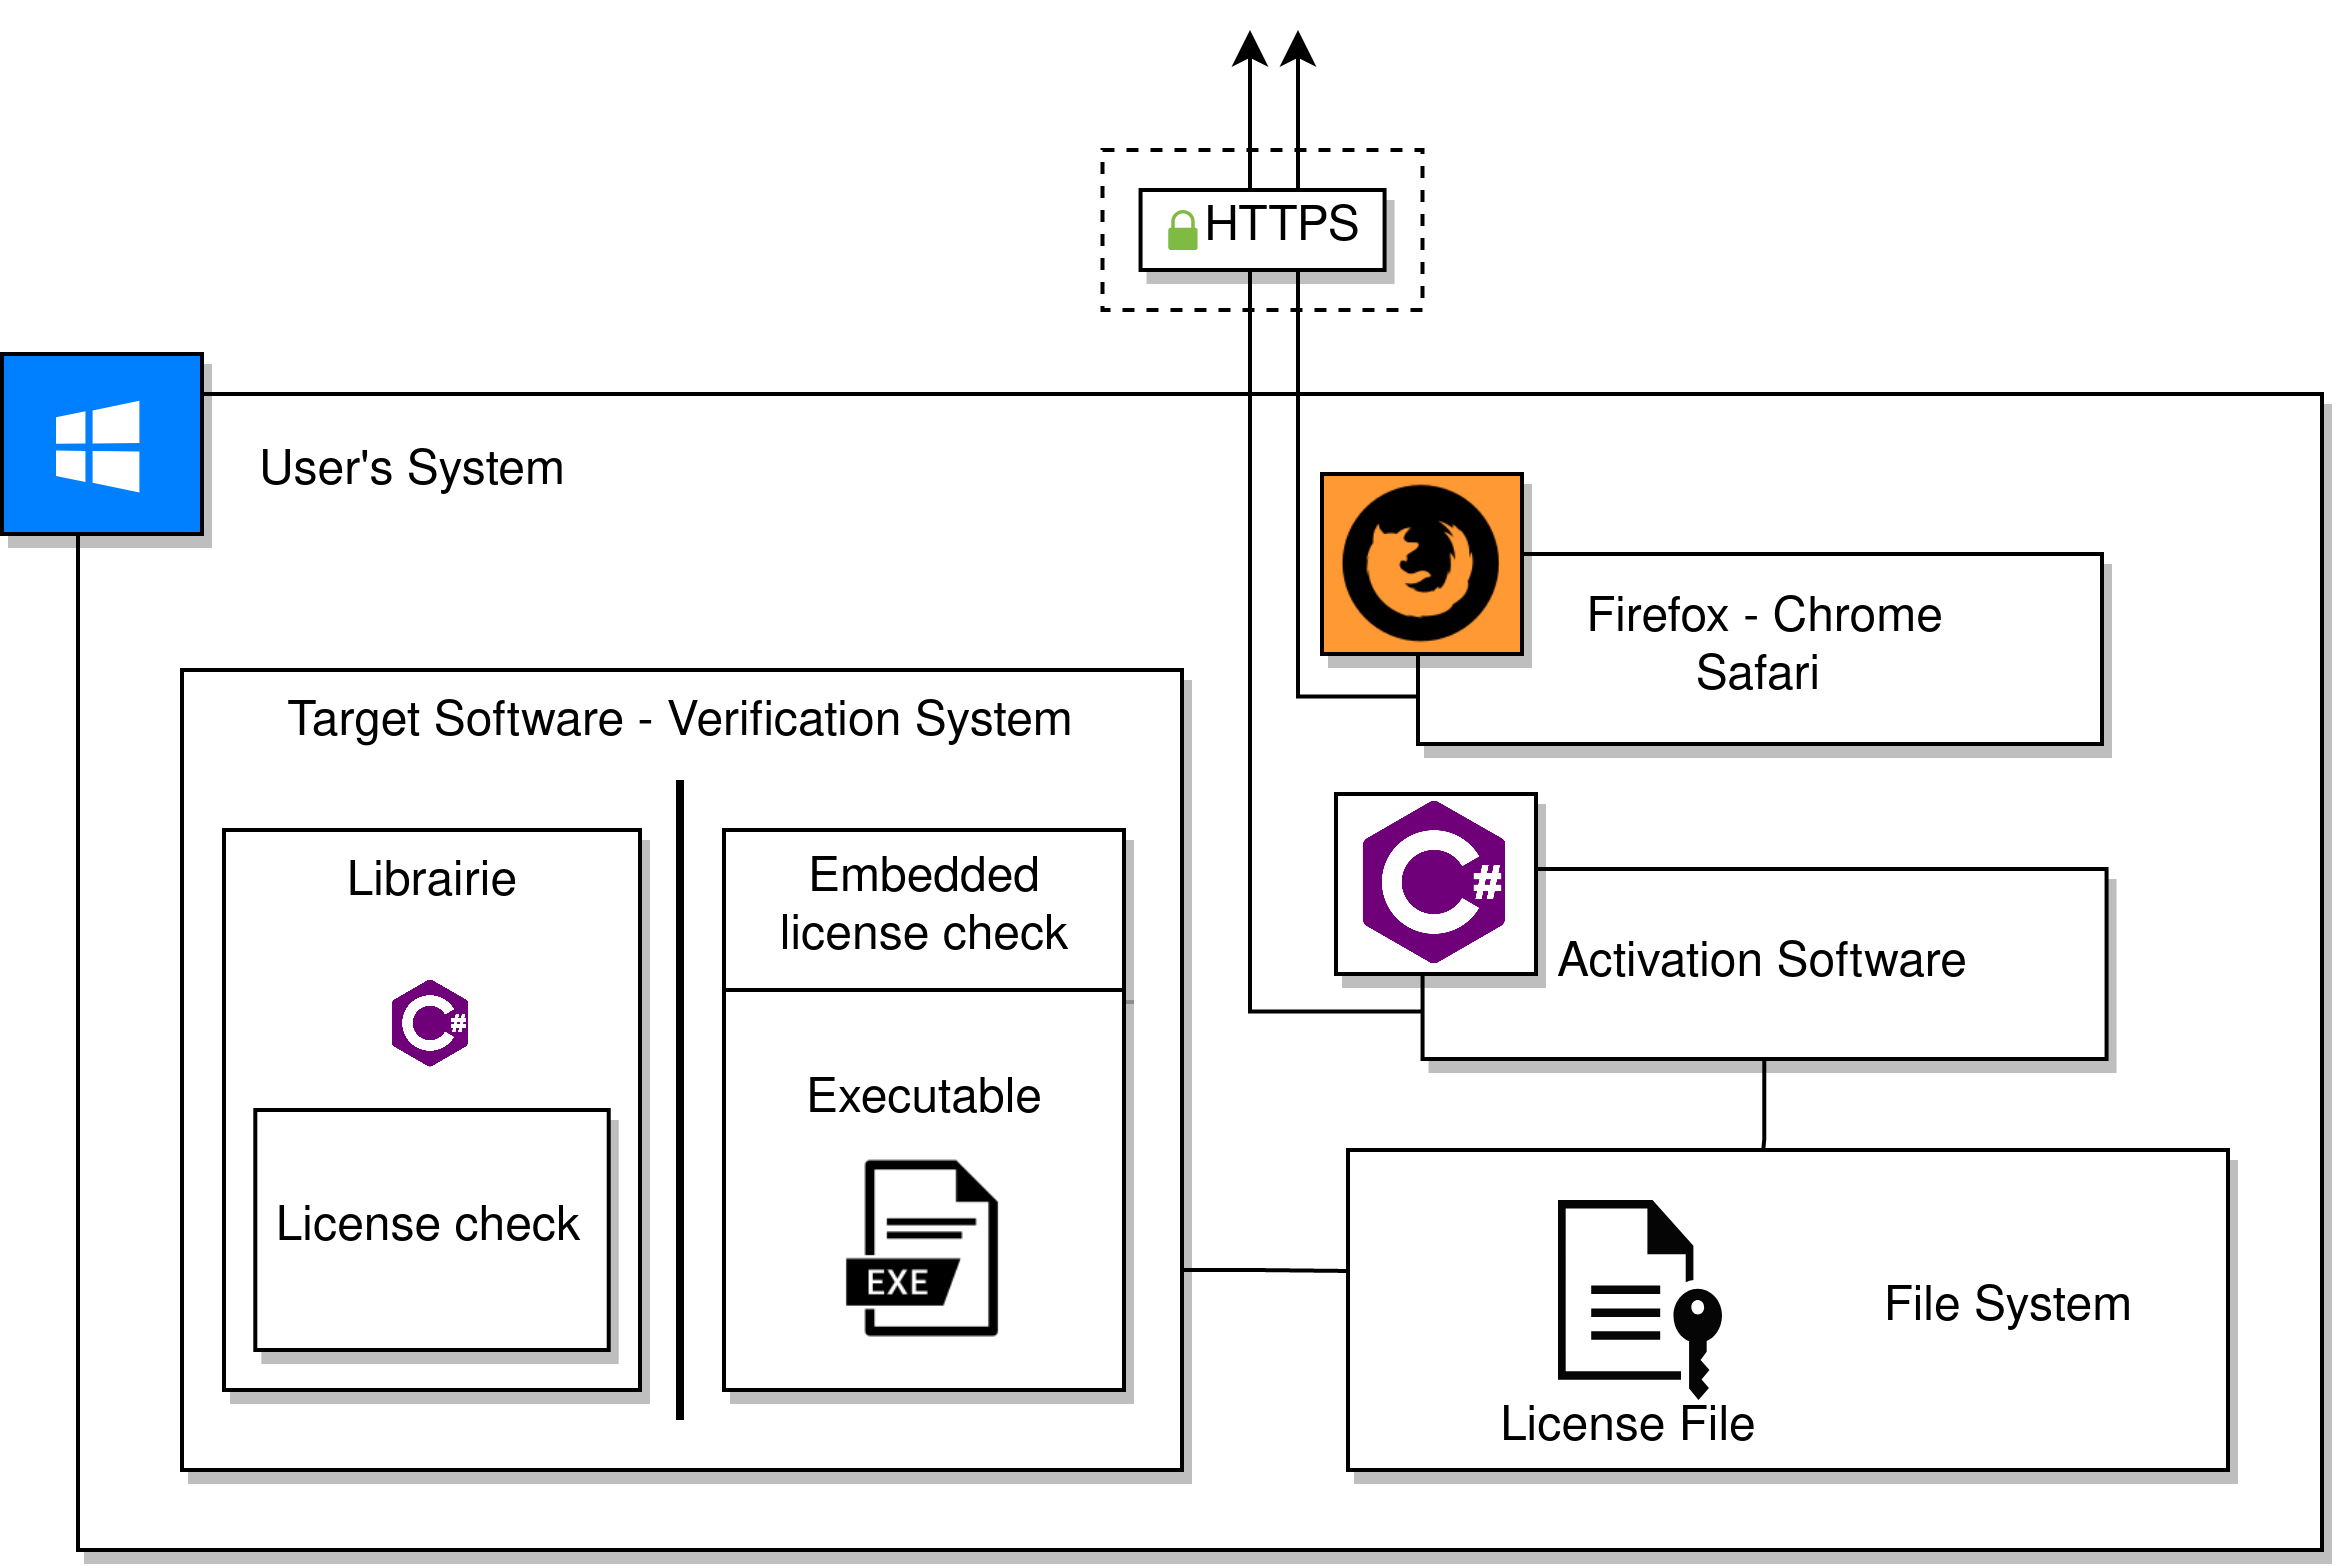
\includegraphics[scale=0.72]{img/DAT-client.png}
    \end{figure}
\end{frame}

\begin{frame}{Solutions techniques}
    \textbf{Plateforme sûre :}
    \begin{itemize}
        \item Chiffrement (HTTPS)
        \item Serveur d'authentification (isolement, configuration)
        \item Hashage des mots de passe (PBKDF)
        \item Sécurisation des bases de données (configuration, requêtes préparées)
        \item API Rest (utilisation de tokens d'authentification)
    \end{itemize}
    \textbf{Génération et vérification de licence :}
    \begin{itemize}
        \item Signature (El Gamal)
        \item Obfuscation
    \end{itemize}
\end{frame}    

\section{Stratégie qualité} % en réponse aux risques

\begin{frame}{Stratégie adoptée}
    \begin{columns}
        \begin{column}{0.54\textwidth}
            \textbf{Actions}
            \begin{itemize}
                \item Gestion et journalisation des bugs
                \item Serveur de tests
                \item Tests unitaires sur le modèle
                \item Tests d'intégration
                \item Tests d'intrusion
            \end{itemize}
        \end{column}
        \begin{column}{0.46\textwidth}
            \textbf{Outils}
            \begin{itemize}
                \item MantisBT
                \item Docker
                \item Jupiter
                \item À définir
                \item Scripts automatiques
            \end{itemize}
        \end{column}
    \end{columns}
\end{frame}

\begin{frame}{Vérification des exigences}
    \begin{itemize}
        \item Définition d'un ordre de priorité sur les erreurs
        \item Rapport concernant les problèmes/failles généré régulièrement
        \item Charte de code et documentation pour un suivi et une maintenabilité du projet
    \end{itemize}
\end{frame}

\section{Organisation du projet} % + planning

\begin{frame}{Affectation des rôles}
    \begin{figure}
        \centering
        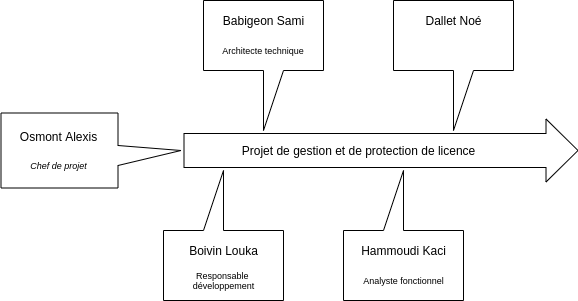
\includegraphics[scale=0.55]{img/schema_role_projet.png}
    \end{figure}
\end{frame}

\begin{frame}{Découpage des tâches}
    \begin{figure}
        \centering
        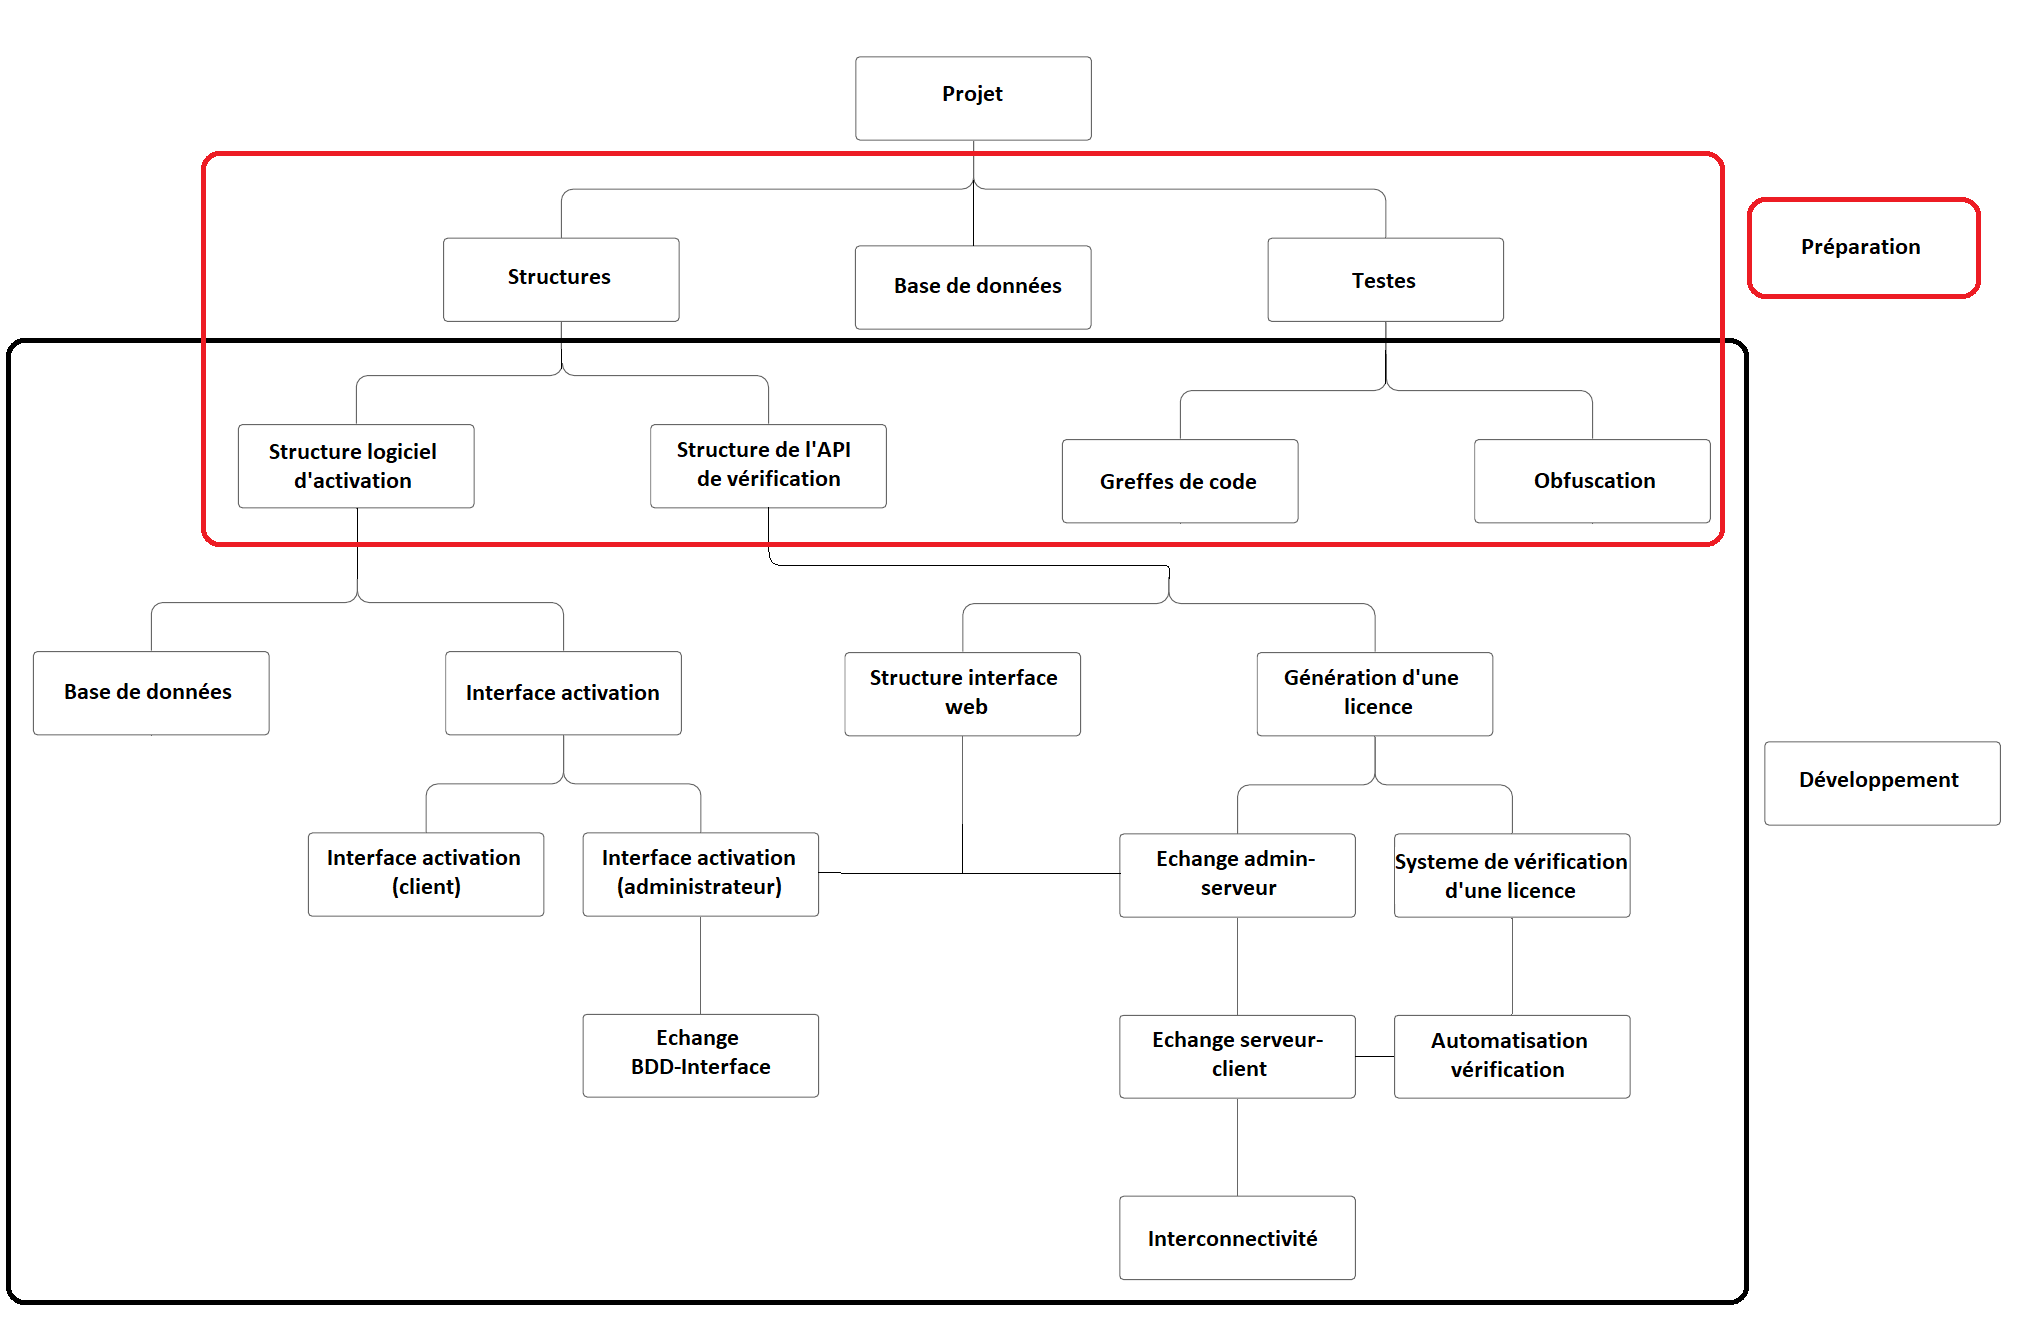
\includegraphics[scale=0.18]{img/organi.png}
    \end{figure}
\end{frame}

\begin{frame}{Diagramme de Gantt}
    \begin{figure}
        \centering
        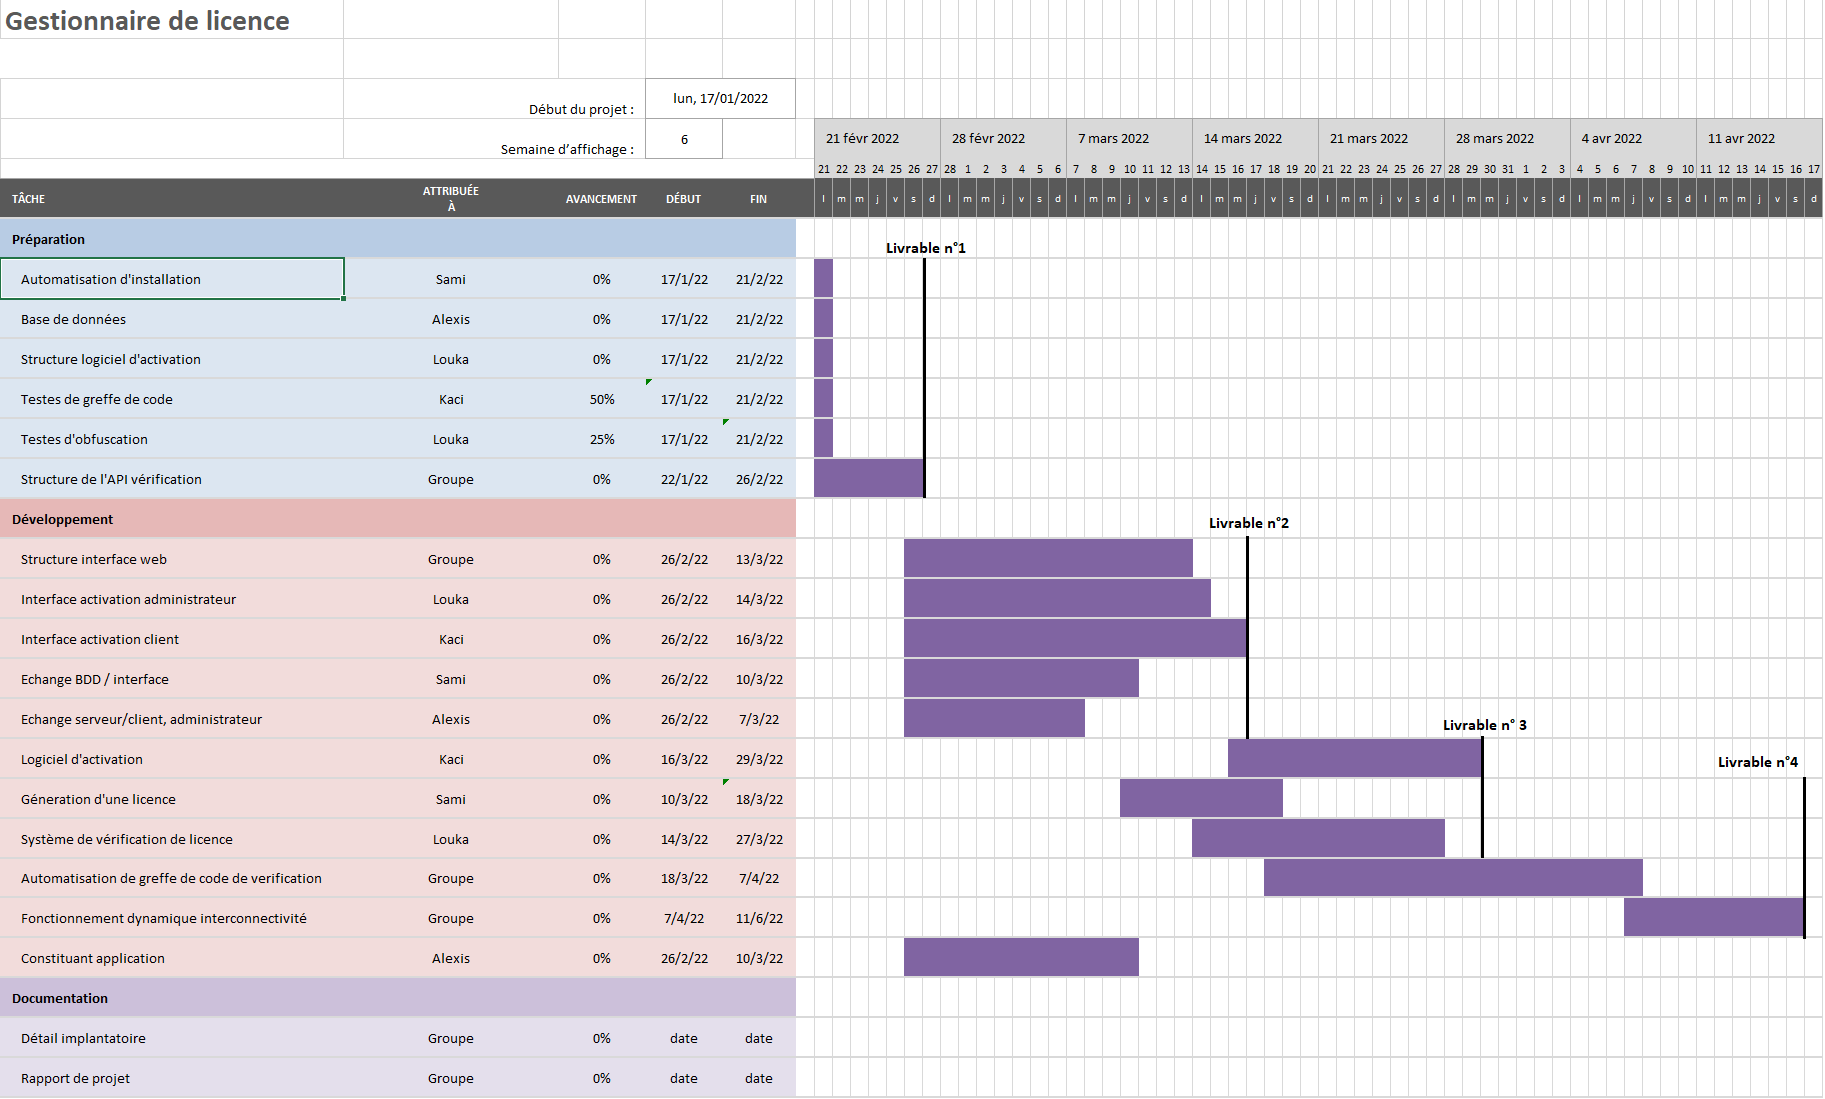
\includegraphics[scale=0.22]{img/Gantt.png}
    \end{figure}
\end{frame}

\section{Risques}

\begin{frame}{Risques principaux}
    \begin{figure}
        \centering
        \vspace{-2mm}
        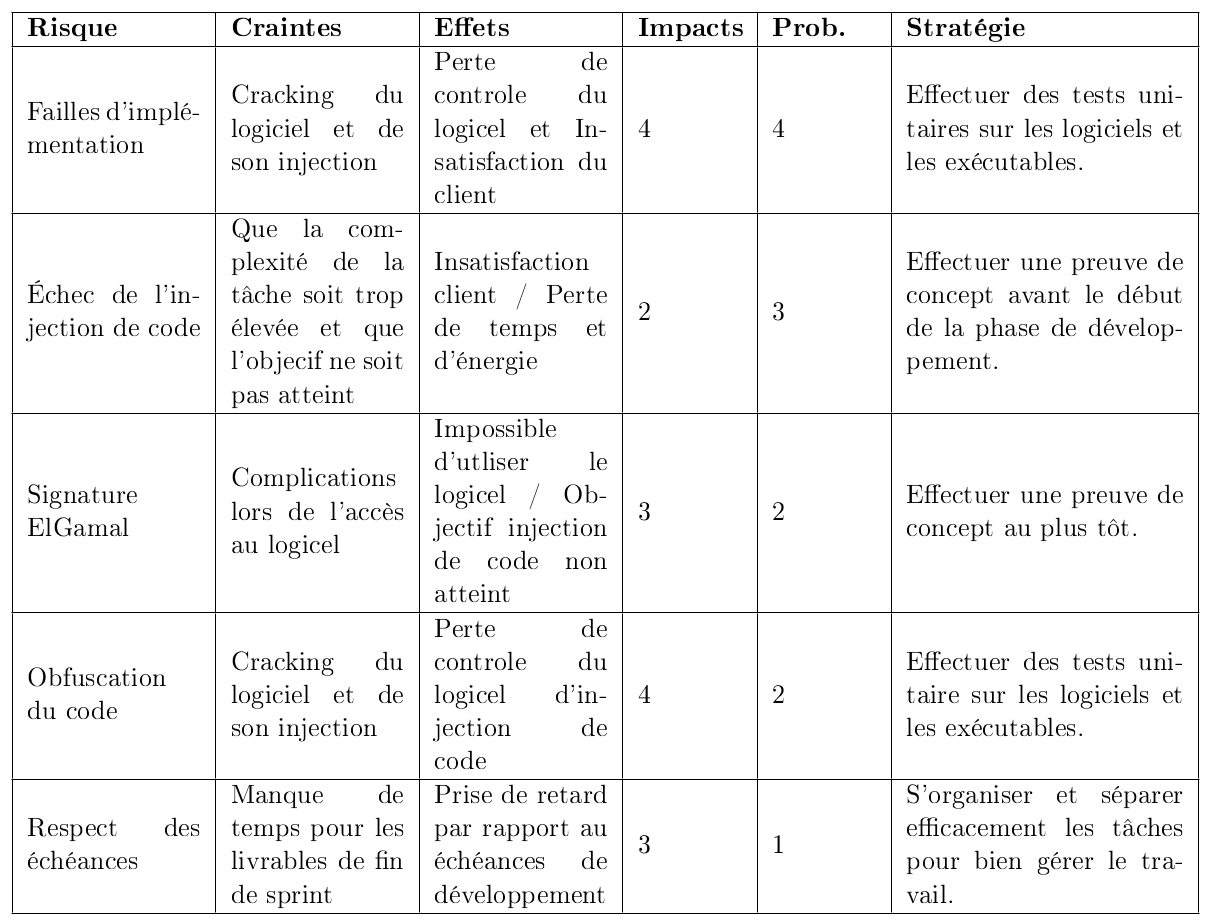
\includegraphics[scale=0.22]{img/risques.png}
    \end{figure}
\end{frame}

% Q&A
\begin{frame}[standout]
    \Huge\textsc{Merci de votre écoute}
    \vfill
    \LARGE\textsc{Questions ?}
\end{frame}

\end{document}

